%%% DOCUMENTCLASS 
%%%-------------------------------------------------------------------------------

\documentclass[
a4paper, % Stock and paper size.
11pt, % Type size.
% article,
% oneside, 
onecolumn, % Only one column of text on a page.
% openright, % Each chapter will start on a recto page.
% openleft, % Each chapter will start on a verso page.
openany, % A chapter may start on either a recto or verso page.
]{memoir}

%%% PACKAGES 
%%%------------------------------------------------------------------------------
\usepackage{amsthm}
\usepackage[utf8]{inputenc} % If utf8 encoding
% \usepackage[lantin1]{inputenc} % If not utf8 encoding, then this is probably the way to go
\usepackage[T1]{fontenc}    %
\usepackage[english]{babel} % English please
\usepackage[final]{microtype} % Less badboxes
\usepackage{dsfont}
% \usepackage{kpfonts} %Font
\usepackage{amsmath,amssymb,mathtools} % Math

% \usepackage{tikz} % Figures
\usepackage{graphicx} % Include figures

%%% PAGE LAYOUT 
%%%------------------------------------------------------------------------------

\setlrmarginsandblock{0.15\paperwidth}{*}{1} % Left and right margin
\setulmarginsandblock{0.2\paperwidth}{*}{1}  % Upper and lower margin
\checkandfixthelayout

%%% SECTIONAL DIVISIONS
%%%------------------------------------------------------------------------------

\maxsecnumdepth{subsection} % Subsections (and higher) are numbered
\setsecnumdepth{subsection}

\makeatletter %
\makechapterstyle{standard}{
	\setlength{\beforechapskip}{0\baselineskip}
	\setlength{\midchapskip}{1\baselineskip}
	\setlength{\afterchapskip}{8\baselineskip}
	\renewcommand{\chapterheadstart}{\vspace*{\beforechapskip}}
	\renewcommand{\chapnamefont}{\centering\normalfont\Large}
	\renewcommand{\printchaptername}{\chapnamefont \@chapapp}
	\renewcommand{\chapternamenum}{\space}
	\renewcommand{\chapnumfont}{\normalfont\Large}
	\renewcommand{\printchapternum}{\chapnumfont \thechapter}
	\renewcommand{\afterchapternum}{\par\nobreak\vskip \midchapskip}
	\renewcommand{\printchapternonum}{\vspace*{\midchapskip}\vspace*{5mm}}
	\renewcommand{\chaptitlefont}{\centering\bfseries\LARGE}
	\renewcommand{\printchaptertitle}[1]{\chaptitlefont ##1}
	\renewcommand{\afterchaptertitle}{\par\nobreak\vskip \afterchapskip}
}
\makeatother

\chapterstyle{standard}

\setsecheadstyle{\normalfont\large\bfseries}
\setsubsecheadstyle{\normalfont\normalsize\bfseries}
\setparaheadstyle{\normalfont\normalsize\bfseries}
\setparaindent{0pt}\setafterparaskip{0pt}

%%% FLOATS AND CAPTIONS
%%%------------------------------------------------------------------------------

\makeatletter                  % You do not need to write [htpb] all the time
\renewcommand\fps@figure{htbp} %
\renewcommand\fps@table{htbp}  %
\makeatother                   %

\captiondelim{\space } % A space between caption name and text
\captionnamefont{\small\bfseries} % Font of the caption name
\captiontitlefont{\small\normalfont} % Font of the caption text

\changecaptionwidth          % Change the width of the caption
\captionwidth{1\textwidth} %

%%% ABSTRACT
%%%------------------------------------------------------------------------------

\renewcommand{\abstractnamefont}{\normalfont\small\bfseries} % Font of abstract title
\setlength{\absleftindent}{0.1\textwidth} % Width of abstract
\setlength{\absrightindent}{\absleftindent}

%%% HEADER AND FOOTER 
%%%------------------------------------------------------------------------------

\makepagestyle{standard} % Make standard pagestyle

\makeatletter                 % Define standard pagestyle
\makeevenfoot{standard}{}{}{} %
\makeoddfoot{standard}{}{}{}  %
\makeevenhead{standard}{\bfseries\thepage\normalfont\qquad\small\leftmark}{}{}
\makeoddhead{standard}{}{}{\small\rightmark\qquad\bfseries\thepage}
% \makeheadrule{standard}{\textwidth}{\normalrulethickness}
\makeatother                  %

\makeatletter
\makepsmarks{standard}{
	\createmark{chapter}{both}{shownumber}{\@chapapp\ }{ \quad }
	\createmark{section}{right}{shownumber}{}{ \quad }
	\createplainmark{toc}{both}{\contentsname}
	\createplainmark{lof}{both}{\listfigurename}
	\createplainmark{lot}{both}{\listtablename}
	\createplainmark{bib}{both}{\bibname}
	\createplainmark{index}{both}{\indexname}
	\createplainmark{glossary}{both}{\glossaryname}
}
\makeatother                               %

\makepagestyle{chap} % Make new chapter pagestyle

\makeatletter
\makeevenfoot{chap}{}{\small\bfseries\thepage}{} % Define new chapter pagestyle
\makeoddfoot{chap}{}{\small\bfseries\thepage}{}  %
\makeevenhead{chap}{}{}{}   %
\makeoddhead{chap}{}{}{}    %
% \makeheadrule{chap}{\textwidth}{\normalrulethickness}
\makeatother

\nouppercaseheads
\pagestyle{standard}               % Choosing pagestyle and chapter pagestyle
\aliaspagestyle{chapter}{chap} %

%%% NEW COMMANDS
%%%------------------------------------------------------------------------------

\newcommand{\p}{\partial} %Partial
% Or what ever you want
%%% TABLE OF CONTENTS
%%%------------------------------------------------------------------------------

\maxtocdepth{subsection} % Only parts, chapters and sections in the table of contents
\settocdepth{subsection}

\AtEndDocument{\addtocontents{toc}{\par}} % Add a \par to the end of the TOC

%%% INTERNAL HYPERLINKS
%%%-------------------------------------------------------------------------------

\usepackage{hyperref}   % Internal hyperlinks
\hypersetup{
	pdfborder={0 0 0},      % No borders around internal hyperlinks
	pdfauthor={Yannick Couzinié} % author
}
\usepackage{memhfixc}   %

%%% THE DOCUMENT
%%% Where all the important stuff is included!
%%%-------------------------------------------------------------------------------

\author{}
\title{Mathematical Statistical Physics}
\theoremstyle{definition}
\newtheorem{definition}{Definition}[chapter]
\newtheorem{example}{Example}[chapter]
\theoremstyle{remark}
\newtheorem{remarks}{Remarks}[chapter]
\newtheorem{notes}{Notes}[chapter]
\theoremstyle{plain}
\newtheorem{theorem}{Theorem}[chapter]
\newtheorem{prop}{Proposition}[chapter]
\newtheorem{lemma}{Lemma}[chapter]
\usepackage{simplewick}
\usepackage{tensor}
\begin{document}
\setlength{\parindent}{0pt}
\maketitle
\tableofcontents

\newpage\chapter{Preliminary stuff}
In the Heisenberg picture of quantum mechanics there are three core principles \begin{enumerate}
	\item Central objects are the observables, which ware realized as operators on a Hilbert space.
	\item Time evolution acts on observables.
	\item Auxiliary objects are the states, realized as vectors on the Hilbert space, used to compute expectation values of observables.
\end{enumerate}
This is a notion heavily based on physical intuition. One can translate these three principles into a mathematical formulation in the following way. \begin{enumerate}
	\item The set of observables is a \textit{C*-algebra} $\mathcal{A}$, namely: \begin{itemize}
		\item $\mathcal{A}$ is an associative algebra.
		\item $\mathcal{A}$ is equipped with a norm such that $\|A\cdot B\| \leq \| A \|\cdot \| B\| $.
		\item it is complete with respect to $\| \cdot \|$.
		\item equipped with an involution $*:\mathcal{A}\rightarrow \mathcal{A}$ such that \begin{align}
		(A^*)^*&=A\\
		(A+\lambda B)^* &= A^* +\overline{\lambda}B^*\\
		(AB)^*&=B^*A^*
		\end{align}
		\item $C^*$-property, i.e. $\|A^*A\|=\|A\|^2$.
	\end{itemize}
\begin{remarks}
	There is a lot to be said about $C^*$-algebras but we will keep it short. \begin{enumerate}
		\item Observables $A\in\mathcal{A}$ are not required to be self-adjoint ($A=A^*$).
		\item In the quantum mechanic setting $\mathcal{H}$ isa Hilbert space, then one takes the ''set of bounded operators'' $\mathcal{A}=\mathcal{L}(\mathcal{H})$.
		\item Physically, there are unbounded observables. At least for self-adjoint ones $A=A'$, one can consider equivalently the unitary correspondents $U=e^{itA}$, since there is a one-to-one correspondence by Stokes' theorem.
		\item $\mathcal{A}$ does not need to have a $\mathds{1}$.
	\end{enumerate}
\end{remarks}
\item A pair $(\mathcal{A},\tau)$ is a $C^*$-dynamical system if $\mathcal{A}$ is a $C^*$-algebra and $\mathbb{R}\ni t\mapsto \tau_t$ is a strongly continuous one-parameter group $*-$automorphism of $\mathcal{A}$: \begin{itemize}
	\item $\tau_t:\mathcal{A}\rightarrow \mathcal{A}$ such that \begin{align}
	\tau_t(A^*)&=(\tau_t(A))^*\\
	\tau_t(A+\lambda B)&=\tau_t(A)+\lambda\tau_t(B)\\
	\tau_t(AB)&=\tau_t(A)\tau_t(B)\\
	\|\tau_t(A)\|&=\|A\|\; .
	\end{align}
	\item $\tau_0(A)=A; \tau_{t+s}=\tau_t(\tau_s(A))$ \; .
	\item For any $A\in \mathcal{A}$, $\| \tau_{t+\varepsilon}(A)-\tau_{t}(A)\|\rightarrow 0 (\varepsilon \rightarrow 0)$, i.e. no uniformity in $A$.
\end{itemize}
\begin{remarks}
	$\tau$ is always generated by a $*$-derivation of the form \begin{align}
	\delta_t:\mathcal{A}&\longrightarrow \mathcal{A}\\
	A&\longmapsto t^{-1}(\tau_t(A)-A)\; .
	\end{align}
	The domain is defined as $D(\delta)=\{A\in\mathcal{A} \mid \lim\limits_{t\rightarrow 0}\delta_t(A) \text{ exists}\}$ for which we then have \begin{align}
	\delta: D(\delta)&\longrightarrow \mathcal{A}\\
	A&\longmapsto \delta(A)=\lim_{t\rightarrow 0}\delta_t(A)\; .
	\end{align}
	Then $\delta$ is a closed, densely defined map such that \begin{align*}
	\mathds{1}\ni D(\delta), \delta(\mathds{1})&=0\\
							\delta(AB)&=\delta(A)B+A\delta(B)\\
							\delta(A^*)&=\delta(A)^*\;  .
	\end{align*}
	In fact, there is a one-to-one correspondence between $\tau_t$ and $\delta$ (Hille-Yoshida).
\end{remarks}
\begin{remarks}
	In the quantum mechanic setting $\mathcal{A}=\mathcal{L}(\mathcal{H})$. The dynamics are generated by a $H\cdot H^*$ on $\mathcal{H}$, namely \begin{align}
	\tau_t(A)=e^{itH}Ae^{-itH}\; .
	\end{align}
	It is a $*$-automorphism by unitarity of $e^{-itH}$ and a strongly continuous group because $t\mapsto e^{-itH}$ is so. The $*$-derivation is given by \begin{align*}
	\delta(A)=\frac{\mathrm{d}}{\mathrm{d}t}\tau_t(A)\mid_{t=0}=i[H,A]\; ,
	\end{align*}
	sometimes written as $\tau_t(A)=e^{i[H,\cdot]t}(A)$.
\end{remarks}
\item Finally, a \underline{state} over $A$ is a positive, normalized linear functional over $A$ \begin{align*}
\omega:\mathcal{A}&\longmapsto \mathbb{C}\\
A\longrightarrow \omega(A)\in\mathbb{C}\; ,
\end{align*}
such that $\omega(A^*A)\geq 0$ (positivity) and $\|\omega \| :=\sup \frac{\|\omega(A)\|}{\|A\|}=1$ (normalization).
\begin{remarks}
	Let us now try to establish some intuition \begin{itemize}
		\item The positivity of the quadratic function $\lambda\mapsto \omega((A+\lambda B)^*(A+\lambda B))$ implies 
		\begin{enumerate}
			\item $\omega(A^*B)=\omega(B^*A)$.
			\item $|\omega(A^*B)|^2\leq \omega(A^*A)\omega(B^*B)$ (Cauchy-Schwarz inequality).
		\end{enumerate}
		\item In the quantum mechanic setting, any normalized vector $\psi\in\mathcal{H}$ defines a state by \begin{align}\omega_{\psi}:\mathcal{A}&\longrightarrow \mathbb{C}\\
		A&\longmapsto \langle \psi, A\psi\rangle \; .\end{align}
		\item Also any density matrix $\varrho = \varrho^*\in \mathcal{L}(\mathcal{H})$ defines a state by \begin{align}
		\omega_{\varrho}:A&\longrightarrow \mathbb{C}\\
		A&\longmapsto \omega_{\rho}(A)=\mathrm{Tr}(\varrho A) \qquad (\mathrm{Tr}(\varrho)=1) \; .
		\end{align}
		\item If $\mathds{1}\in\mathcal{A}$, then $\omega$ is normalized $\Leftrightarrow$ $\omega(\mathds{1})=1$.
		\end{itemize}
\end{remarks}
\end{enumerate}
It turns out that $\mathcal{A}$ may have inequivalent representations, corresponding to thermodynamically different situations. A representation of the $C^*$-algebra $A$ on a Hilbert-space $\mathcal{H}$ is a $*$-morphisms
$\pi:\mathcal{A}\longrightarrow \mathcal{L}(\mathcal{H})$, namely \begin{align}
\pi(A\cdot B)&=\pi(A)\pi(B) \\
\pi(A+\lambda B)&=\pi(A)+\lambda\pi(B)\\
\pi(A^*)&=(\pi(A))^*\;.
\end{align}
$\pi_1,\pi_2$ are called equivalent if there is a unitary map \begin{align}
U:\mathcal{H}_1\rightarrow \mathcal{H}_2 \text{ s.t. } U\Pi_1(A)=\Pi_2(A)U\quad \forall A\in \mathcal{A}\; .
\end{align}
Now given a $\pi$ on $\mathcal{H}$ and any normlized vector $\xi\in\mathcal{H}$, then the map \begin{align}
\omega_{\xi}:\mathcal{A}&\longrightarrow \mathbb{C}\qquad \omega_{\xi}(A)=\langle\xi,\pi(A)\xi\rangle \; ,
\end{align}
defines a state on the algebra. Given a state $\omega$ on $\mathcal{A}$, there exists a $\mathcal{H}\omega$, a representation $\pi_{\omega}:\mathcal{A}\rightarrow \mathcal{H}\omega$ and a normalized $\Omega_{\omega}\in\mathcal{H}\omega$ such that \begin{align}
\omega(A)=\langle\Omega_{\omega},\pi_{\omega}(A)\Omega_{\omega}\rangle \quad \text{''GNS construction''.}
\end{align}
We will be mainly using two topologies \begin{enumerate}
	\item In $A$: $A_n\rightarrow A$ if $\|A_n-A\|\rightarrow 0$. 
	\item In a representation where $A$ is represented as $\mathcal{L}(\mathcal{H})$ there: uniform convergence, strong convergence, weak convergence apply as usual, outside of representations, these terms do not make sense.
\end{enumerate}
\begin{remarks}
	On the set of states over $\mathcal{A}$, designated by $\varepsilon(\mathcal{A})$, one has \begin{itemize}
		\item $\varepsilon(\mathcal{A})$ is a convex set. $\omega_1,\omega_2\in\varepsilon(\mathcal{A})$ then $\omega=\lambda\omega_1+\mu\omega_2\in\varepsilon(\mathcal{A})$.
		\item $\varepsilon(\mathcal{A})$ is weakly-$*$ compact (if $\mathcal{A}$ has an identity), namely every sequence $(\omega_n)_{n\in\mathcal{N}}$ of states in $\mathcal{A}$ has convergent subsequences (in the weak-$*$-topology) $\exists(n_k)_{k\in\mathcal{N}}:\omega_{n_k}(A)\rightarrow \overline{\omega}(A)$.
	\end{itemize}
In particular: A sequence of finite volume thermal equilibrium states always have infinite-volume limit points. As we shall see later, the uniqueness of the infinity point can be takes as a characterization of phase transitions.
\end{remarks}
\chapter{Ideal gases}
The ideal gas is a gas of non-interacting particles. The thermodynamic limit (TDL) is usually obtained by taking $N$ particles in a  finite volume $\Lambda\in \mathbb{R}^d$ and letting $N\rightarrow\infty$, $\Lambda\rightarrow\mathbb{R}^d$ such that \begin{align}
N/|\Lambda|\rightarrow \varrho \qquad \text{ with } \qquad 0<\varrho < \infty.
\end{align}
There are two types of indistinguishable particles in nature \begin{enumerate}
	\item Bosons have a symmetric wave function.
	\item Fermions have an antisymmetric wavefunction.
\end{enumerate}
A Hilbert space carrying an arbitrary number of particles is a Fock space built upon the one-particle Hilbert space. Action of the symmetric group $S_n$ on $\otimes^N\mathcal{H}$. \begin{align}
P_{\sigma}:\psi_1\otimes \cdots \otimes \psi_N \longmapsto \psi_1{\sigma^{-1}(1)\otimes \cdots \otimes \psi_{\sigma^{-1}(N)}}\; ,
\end{align}
for any $\sigma\in S_n$ (check $P_{\sigma\sigma'}=P_{\sigma}\circ P_{\sigma'}$ and so on) and now \begin{align}
\mathcal{H}_{s/a}^{N}&:=\{\psi\in\otimes^N\mathcal{H}:P_{\sigma}\psi=\delta(\sigma)\psi \text{ for any } \sigma\in S_n\}\; ,\\\delta(\sigma)&=\begin{cases}
1 &\text{ if ''s'' (Bosons)}\\
-1 &\text{ if ''a'' (Fermions)}
\end{cases}\; .
\end{align}
Furthermore one has $\mathcal{H}_{s/a}^0:=\mathbb{C}$ with unit vector $\Omega$, called ''vacuum''. Now the Fock space is given by \begin{align}
\mathcal{F}_{s/a}(\mathcal{H})=\bigoplus_{N\in\mathcal{N}\cup\{0\}}\mathcal{H}_{s/a}^N\; ,
\end{align}
$\psi\in\mathcal{F}_{s/a}(\mathcal{H})$ is represented as $(\psi^N)_{N\in\mathcal{N}\cup\{0\}}=(\psi^0,\psi^1,\ldots)$ where $\psi^N\in\mathcal{H}^N_{s/a}$ with the norm given by \begin{align}
\|\psi\|^2_{\mathcal{F}_{s/a}(\mathcal{H})}=\sum_{N\geq 0}\|\psi^N\|^2_{\otimes^N\mathcal{H}}\; .
\end{align}
\begin{remarks}
	\begin{itemize}
		\item This sum has to be convergent, thus the series elements have to decrease in value. Sinc ehte proability to have more than $M$ particles is given by taking the sum $\sum_{N\geq M}\|\psi^N\|^2_{\otimes^N\mathcal{H}}$. So Fock space does not describe the infinite particle state as for $M\rightarrow\infty$ the state would always be zero. One can only take the TDL.
		\item The number operator is given by $(N\psi)^N=N\psi^N$ for any $N\in \mathcal{N}$.
		\item Second quantization: If $A:\mathcal{H}\rightarrow \mathcal{H}$ is a linear operator then define $\Gamma(A),\mathrm{d}\Gamma(A):\mathcal{H}_{s/a}^N\rightarrow \mathcal{H}_{s/a}^N$ for any $N$ where \begin{align}
		\Gamma(A)&=A\otimes \cdots \otimes A\\
		\mathrm{d}\Gamma(A)&=\sum_{j=1}^N\mathds{1}\otimes\cdots\otimes \mathds{1}\otimes \underbrace{A}_{\text{j-th position}}\otimes \mathds{1}\cdots \otimes \mathds{1}\;,
		\end{align}
		with which one has $N=\mathrm{d}\Gamma(\mathds{1})$. Also if $A$ is self-adjoint then $\frac{\mathrm{d}}{\mathrm{d}t}\Gamma(e^{itA})\mid_{t=0}=i\mathrm{d}\Gamma(A)$ i.e. $\Gamma(e^{itA})=e^{itd\Gamma(A)}$.
	\end{itemize}
\end{remarks}
The core concepts of Fock spaces are those of annihilation and creation operators. \begin{itemize}
	\item Annihilation operators: For $\varphi\in\mathcal{H}$ one defines \begin{align}
	b(\varphi):\otimes^N\mathcal{H}&\longrightarrow \otimes^{N-1}\mathcal{H}\\
	b(\varphi)(\psi_1\otimes\ldots\otimes\psi_N)&=\sqrt{N}\langle \varphi,\psi_1\rangle_{\mathcal{H}}~\psi_2\otimes\ldots\otimes\psi_N\\
	b(\varphi)\Omega &= 0\; .
	\end{align}
	Since $b(\varphi):\mathcal{H}_{s/a}^N\rightarrow \mathcal{H}_{s/a}^{N-1}$ for any $N$, it extends to a map $b(\varphi):\mathcal{F}_{s/a}(\mathcal{H})\rightarrow \mathcal{F}_{s/a}(\mathcal{H})$.
	\item Creation operators: For $\varphi\in\mathcal{H}$ one defines \begin{align}
	b^*(\varphi)\psi^{N-1}&=\frac{1}{\sqrt{N}}\sum_{k=1}^{N}(\pm 1)^{k-1}P_{\pi_k}(\varphi\otimes \psi^{N-1}) \text{ where $\pm$ is for $s/a$ and}\\
	\pi_k^{-1}&=(k,1,2,\cdots,k-1,k+1,\cdot,N)\; .
	\end{align}
	This can be interpreted as inserting a particle $\varphi$ into each position and average over the possible positions, that's what $P_{\pi_k}$ does, inserting into the $k$-th position. Proving this exactly is cumbersome.
	\end{itemize}
\begin{remarks}
	\begin{itemize}
		\item $b^*(\varphi)=(b(\varphi))^*$.
		\item $\varphi\mapsto b(\varphi)$ is anti-linear, i.e. $\varphi\mapsto b^*(\varphi)$ is linear.
		\item The following commutation law holds $Nb(\varphi)=b(\varphi)(N-1)$. 
		\item If $U:\mathcal{H}\rightarrow\mathcal{H}$ is unitary: $\Gamma(U)b^*(\varphi)\Gamma(U)^*=b^*(U\varphi)$.
		\item The following commutation relations hold on $\mathcal{F}_s(\mathcal{H})$ (CCR) \begin{align}
		[b(\varphi),b^*(\psi)]&=\langle\varphi,\psi\rangle\mathds{1}\\
		[b(\varphi),b(\psi)]&=[b^*(\varphi),b^*(\psi)]=0\; .
		\end{align}
		\item Canonical anticommutatoin relation on $\mathcal{F}_a(\mathcal{H})$ (CAR)\begin{align}
		\{b(\varphi),b^{\dagger}(\psi)\}&=\langle\varphi,\psi\rangle \mathds{1}\\
		\{b(\varphi),b(\psi)\}&=\{b^*(\varphi),b^*(\psi)\}=0\; ,
		\end{align}
		where $\{A,B\}=AB+BA$.
	\end{itemize}
\end{remarks}
\section{Fermions}
The (CAR) relatoins indicate that the fermionic creation/anihilation operators are a representation of the abstract algebra $CAR(\mathcal{H})$, defined as the $C^*$-algebra generated by $\mathds{1}, a(\varphi), \varphi\in\mathcal{H}$ satisfying: \begin{itemize}
	\item $\varphi\mapsto a(\varphi)$ is antilinear.
	\item $\{a(\varphi),a(\psi)^*\}=\langle\varphi,\psi\rangle$ ; $\{a(\varphi),a(\psi)\}=0=\{a(\varphi)^*,a(\psi)^*\}$. 
\end{itemize}
Since \begin{align}
(a(\varphi)^*a(\varphi))^2=&a(\varphi)^*\{a(\varphi),a(\varphi)^*\}a(\varphi)\\
=&\|\varphi\|^2a(\varphi)^*a(\varphi)\mid \text{ by the C*-property}\\
=&\|a(\varphi)^*a(\varphi)\|^2=\|\varphi\|^2\|a(\varphi)^*a(\varphi)\|\\
\Rightarrow&\|a(\varphi)^*\|=\|\varphi\|\; ,
\end{align}
so that the map $\varphi\mapsto a(\varphi)^*$ is continuous. \begin{remarks}
	\begin{itemize}
		\item If $h$ is a pre-Hilbert space, with $\overline{h}=\mathcal{H}$, then $CAR(h)=CAR(\mathcal{H})$.
		\item $CAR(\mathcal{H})$ is unique up to $*$-isomorphisms.
	\end{itemize}
\end{remarks}
Consider Thermal equilibrium in a finite volume $\Lambda \subset C\mathbb{R}^d$. \textit{Gibbs state} at inverse temperature $0<\beta<\infty$ and chemical potential $\mu\in\mathbb{R}$ is given by \begin{align}
w_{\beta,\mu}(A):=Z^{-1}_{\beta,\mu} \mathrm{Tr}(e^{-\beta K_{\mu}}A)\; ,
\end{align}
where $A\in \mathrm{CAR}(\mathcal{H}_1)$ and $K_{\mu}=\mathrm{d}\Gamma(H-\mu\mathds{1})=\mathrm{d}\Gamma(H)-\mu\mathcal{N}$ and \begin{align}
Z_{\beta,\mu}=\mathrm{Tr}(e^{-\beta K_{\mu}})\; ,
\end{align}
wheneer $\exp(-\beta K_{\mu})\in I_1(\mathcal{F}_a(\mathcal{H}_1))$ (trace-class operator).
\begin{lemma}
	$\exp(-\beta H)\in I_1(\mathcal{H}_1)\Leftrightarrow \exp(-\beta K_{\mu})\in I_1(\mathcal{F}_a(\mathcal{H}_q))\forall\mu\in \mathbb{R}$.
\end{lemma}
\begin{example}
	$\Lambda=[-L/2,L/2], \mathcal{H}_1=L^2(\Lambda), H=-\Delta_L$.
\end{example}
\underline{But} $-\Delta$ on $\mathbb{R}^d$ has purely absolutely continuous spectrum so $\exp(\Delta)$ cannot be trace-class. Defining the activity Z as \begin{align}
Z=e^{\beta\mu}\; ,
\end{align}
one can find the following relation \begin{align}
\exp(-\beta K_{\mu})&=\gamma(\exp(-\beta(H-\mu\mathds{1})))=Z\Gamma(\exp(-\beta H))\\
e^{-\beta K_{\mu}}b^{\#}(\varphi)&=zb^{\#}(e^{-\beta H}\varphi)e^{-\beta K_{\mu}}\label{eqn::hashtag_dat_shit}\; ,
\end{align}
whereby the hashtag is a placeholder for nothing or dagger.
\begin{prop}
	If $\exp(-\beta H)\in I_1(\mathcal{H}_1)$, then the Gibbs states are given by\begin{align}
	\omega_{\beta,\mu}(a^{*}(\varphi)a(\psi))&=\langle \psi, Ze^{-\beta H}(1+Ze^{-\beta H})^{-1}\varphi\rangle\\
	\omega_{\beta,\mu}(a^*(\varphi))&=0=\omega_{\beta,\mu}(a(\varphi))\; .
	\end{align}
\end{prop}
\begin{proof}
	By Eq. \eqref{eqn::hashtag_dat_shit} one has \begin{align}
	\omega_{\beta,\mu}(a^{*}(\tilde{\varphi})a(\psi))&=Z^{-1}_{\beta,\mu}\mathrm{Tr}(b^*(Ze^{-\beta H}\tilde{\varphi})e^{-\beta K_{\mu}}b(\varphi)) \mid \text{cyclicity of trace}\\
	&=\omega_{\beta,\mu}(a(\psi)a^*(Ze^{-\beta H}\tilde{\varphi})) \mid \text{use CAR}\\
	&=-\omega_{\beta,\mu}(a^*(Ze^{-\beta H}\tilde{\varphi})a(\psi))\langle \psi, Ze^{-\beta H}\tilde{\varphi}\rangle\\
	\Rightarrow \omega_{\beta,\mu}(a^*((\mathds{1}+Ze^{-\beta H})\tilde{\varphi})a(\psi))&=\langle \psi, Ze^{-\beta H} \tilde{\varphi}\rangle\; ,
	\end{align}
	and hence the first term of the claim, since $Ze^{-\beta H}>0$ implies that $(\mathds{1}+Ze^{-\beta H})$ is invertible.\\
	If $\psi$ is such that $\mathcal{N}\psi= N\psi$ (i.e. finite particle number) then \begin{align}
	\langle \psi,e^{-\beta K_{\mu}}\psi\rangle &={N}^{-1}\langle \psi , e^{-\beta K_{\mu}}b(\varphi)\mathcal{N}\psi\rangle\\
	&= N^{-1}\langle \psi, (\mathcal{N}+1)e^{-\beta K_{\mu}}b(\varphi)\psi\rangle\\
	&=\frac{N+1}{N}\langle \psi, e^{-\beta K_{\mu}}b(\varphi)\psi\rangle\\
	\Rightarrow \langle \psi,e^{-\beta K_{\mu}}\psi\rangle&=0\; .
	\end{align}
	Computing $\mathrm{Tr}(e^{-\beta K_{\mu}}b(\varphi))$ in a basis such vectors proves the claim. Now: By a similar argument \begin{align}
	\omega_{\beta,\mu}(a^*(\varphi_1)\cdots a^{*}(\varphi_n)a(\psi_m)\cdot a(\psi_1))=\delta_{n,m}\det\left(\{\langle\psi_i,\varrho\psi_j\rangle\}_{i,j=1}^{n}\right)\; ,	\end{align}$\text{where }\varrho = Ze^{-\beta H}(\mathds{1}+Ze^{-\beta H})^{-1}$.
\end{proof}
\begin{remarks}
	The \textit{2n-point function} is expressed in terms of the 2-point function $\langle \psi, Ze^{-\beta H}(\mathds{1}+Ze^{-\beta H})^{-1}\varphi\rangle$ called \textit{Gaussian state} or \textit{quasi-free state}.
\end{remarks}
\begin{remarks}
	The crucial property used in this calculation, expressed in Eq. \eqref{eqn::hashtag_dat_shit}, is the \textit{KMS condition}: \begin{align}
	\omega_{\beta,\mu}(BA)&=\omega_{\beta,\mu}(A\underbrace{\tau_{i\beta}(B)}_{e^{\beta K_{\mu}}Be^{-\beta K_{\mu}}})\; .
	\end{align}
\end{remarks}
Take the thermodynamic limit, which means here that $\mathcal{H}=L^2(\mathbb{R}^d)$, then one has to take the limit of the operators \begin{align}
(H\psi)(x)=(-\Delta \psi)(x)=(2\pi)^{-d/2}\int |\xi|^2\hat{\psi}(\xi)e^{i\xi\cdot x}\mathrm{d}\xi\; .
\end{align}
How can one evaluate this? The dynamics on $CAR(\mathcal{H})$ are given by $\tau_t(a^{\#}(\varphi))=a^{\#}(e^{-itH}\varphi)$. As one does per usual one takes the well understood finite case $f(-\Delta_L)$ which converges to $f(-\Delta)$ strongly for any bounded, continuous function f. This applies to $e^{-itx}$, $e^{-\beta x}$, $Ze^{-\beta x}(1+Ze^{-\beta x})^{-1} (\text{for }x>0)$.
\begin{theorem}
	Let $\omega_{\beta,\mu}^2$ be the Gibbs state associated to $H_l=-\Delta_L$ on $CAR(\mathcal{H}_L)$. Then \begin{align*}
	\omega_{\beta,\mu}^L(A)\overset{}{\longrightarrow}\omega_{\beta,\mu}(A) \qquad (L\rightarrow \infty)\; ,
	\end{align*}
	for any $A\in CAR(\mathcal{H}_{L})$ and any $L$, where $\omega_{\beta,\mu}$ is the quasi-free state over $CAR(\mathcal{H})$ with the two-point function \begin{align}
		\omega_{\beta,\mu}(a^*(\varphi)a(\psi))=(2\pi)^{-d/2}\int\overline{\psi(\xi)}\frac{Ze^{-\beta |\xi|^2}}{1+Ze^{-\beta|\xi|^2}}\hat{\varphi}(\xi)\mathrm{d}\xi\; .
	\end{align}
\end{theorem}
\begin{proof}
	It suffices to proe the statement for the two-point function. But this follows from the weak convergence of \begin{align}
	Ze^{-\beta(-\Delta_L)}(\mathds{1}+Ze^{-\beta(-\Delta_L)})\overset{w}{\longrightarrow}Ze^{-\beta(-\Delta)}\left(\mathds{1}+Ze^{-\beta(-\Delta)}\right)^{-1}\; ,
	\end{align}
	for a proof refer to exercise sheet 1.
\end{proof}
\begin{remarks} This theorem has obviously a lot of interesting implications, amongst other things
	\begin{itemize}
		 \item Given $\beta,\mu$, the limit of $\omega_{\beta,\mu}^L$ exists and it is unique and $\omega_{\beta,\mu}$ defines the thermal equilibrium state on $CAR(L^2(\mathbb{R}^d))$.
		 \item Density of the free Fermi gas \begin{align}
		 \varrho(\beta,\mu)&=\lim_{L\rightarrow\infty}L^{-d}\sum_{n\geq 1} \omega_{\beta,\mu}^L(\underbrace{a^{\dagger}(\psi_n)a(\psi_n)}_{\mathcal{N}})\\
		 &=(2\pi)^{d/2}\int \frac{Ze^{-\beta}|\xi|^2}{1+Ze^{-\beta|\xi|^2}}\mathrm{d}\xi\; ,
		 \end{align}
		 where $(\psi_n)_{n\in\mathcal{N}}$ is a basis of $\mathcal{H}_L$. This means that the momentum density distribution \begin{align}
		 0\leq \frac{Ze^{-\beta|\xi|^2}}{1+Ze^{-\beta|\xi|^2}}\leq 1\; ,
		 \end{align}
		 and its limit as $\beta\rightarrow\infty$ (i.e. $T\rightarrow 0$) \begin{align}
		 \lim_{\beta\rightarrow \infty}\frac{1}{1+e^{\beta(|\xi|^2-\mu}}=\begin{cases}
		 0 :& \text{ if }|\xi|^2 > \mu\\
		 1 :& \text{ if }|\xi|^2< \mu \; .
		 \end{cases}
		 \end{align}
		 This is illustrated in Fig. \ref{fermidirac}. \begin{figure}\centering
		 	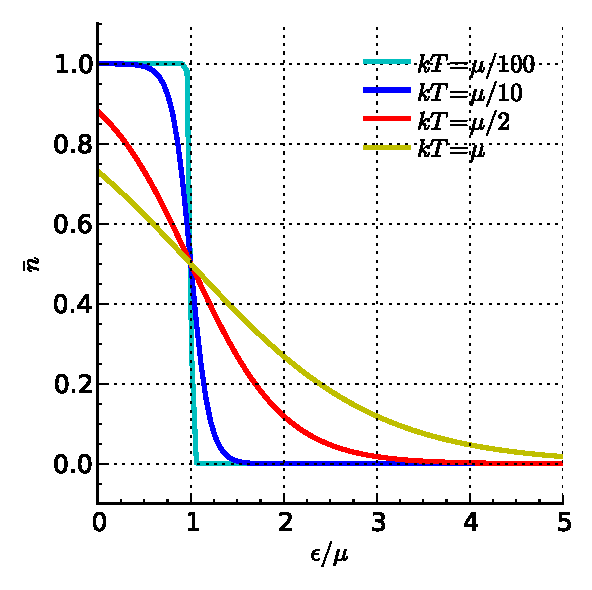
\includegraphics[scale=1]{fermidirac.pdf}
		 	\caption{Fermi-Dirac distribution [stolen; By Krishnavedala - Own work, CC BY-SA 3.0, \texttt{https://commons.wikimedia.org/w/index.php?curid=15478733}]\label{fermidirac}.}
		 \end{figure}
	 \item $\omega_{\beta,\mu}$ having an infinite number of particles cannot be given by a vector or density matrix in $\mathcal{F}_a(L^2(\mathbb{R}^d))$. There is the famous Araki-Wyss representation associated to $\omega_{\beta,\mu}$, namely to $\varrho=\frac{Ze^{-\beta H}}{\mathds{1}+Ze^{-\beta H}}$. \begin{align}
	 H_{\varrho}=\mathcal{F}_a (\mathcal{H}) \otimes \mathcal{F}_a(\mathcal{H}) \qquad \omega_{\varrho}=\omega\otimes\omega \\
	 \pi(a^*(\varphi))=b^*(\sqrt{1-\varrho}\varphi)\otimes \mathds{1}+(-\mathds{1})^{\mathcal{N}}\otimes b(\sqrt{\varrho}\varphi)\; .
	 \end{align}
	 If the density is a projection, i.e. $\varrho=\varrho^2$ (for us that means $\beta=\infty$, as is clearly visible in Fig. \ref{fermidirac}., then the two Fock-spaces have the interpretation: $\text{particles}\otimes\text{antiparticles}$. Check ($\mathcal{H}_\varrho,\Omega_{\varrho},T_{\varrho}$) is the GNS representation of $\omega_{\beta,\mu}$: \begin{align}
	 \langle \Omega_{\varrho},\pi_{\varrho}(a^*(\varphi)a(\varphi))\Omega_{\varrho}\rangle&=\langle \Omega\otimes \Omega,\left((-\mathds{1})^{\mathcal{N}}\otimes b(\sqrt{\varrho}\varphi)\right)\left((-\mathds{1})^{\mathcal{N}}\otimes b^*(\sqrt{\varrho}\psi)\right)\Omega\otimes \Omega)\\
	 &=\langle \Omega,b(\sqrt{\varrho}\varphi)b^*(\sqrt{\varrho}\psi)\Omega\rangle\\
	 &=\langle \sqrt{\varrho}\psi,\sqrt{\varrho}\varphi\rangle+\langle \Omega ,b^*(\sqrt{\varrho}\psi)b(\sqrt{\varrho}\varphi)\Omega\rangle\\
	 &=\langle \psi,\varrho\varphi\rangle=\omega_{\beta,\mu}(a^*(\varphi)a(\varphi))
	 \end{align}
	\end{itemize}
\end{remarks}
\section{Bosons}
The main difference to Fermions is that $b(\varphi),b^*(\psi)$ are unbounded on Fock space so they cannot generate a $C^*$-algebra. But $\Phi(\psi):=\frac{1}{\sqrt{2}}(b(\psi)+b^*(\psi))$ can be realised as a self-adjoined operator on $\mathcal{F}_s(\mathcal{H})$, and hence \begin{align}
W(t\psi):=\exp(it\Phi(\psi))\qquad (t\in\mathbb{R})\; ,
\end{align}
is a strongly continuous group of unitary operators. if $\mathcal{H}$ is a separable Hilbert space, the Weyl algebra $CCR(\mathcal{H})$ is the $C^*$-algebra generated by $\{W(\psi),\psi\in\mathcal{H}\}$ such that \begin{itemize}
	\item $W(\psi)=W(-\psi)^*$.
	\item $W(\varphi)W(\psi)=e^{-\frac{i}{2}\mathrm{Im}(\langle\varphi,\psi\rangle)}W(\varphi+\psi)$.
\end{itemize}
\begin{remarks}
	There are some remarks, mostly analogous to the Fermion case, to be made \begin{itemize}
		\item Again: $CCR(\mathcal{H})$ is unique up to $*$-isomorphisms.
		\item Here if $h$ is a pre-Hilbert space, with $\overline{h}=\mathcal{H}$. Then $CCR(h)=CCR(\mathcal{H})$ iff $h=\mathcal{H}$.
		\item $W(0)=\mathds{1}$, $W(\psi)$ is unitary for all $\psi\in\mathcal{H}$.
		\item $\|W(\psi)-\mathds{1}\|=2$ for all $\psi\neq 0$ i.e. \underline{no} norm continuity in $\psi\mapsto W(\psi)$.
		\item The map $\psi\mapsto W(\psi)$ is called the \underline{Weyl quantization}.
	\end{itemize}
\end{remarks}
The finite volume thermal Gibbs state is again given by \begin{align}
\omega_{\beta,\mu}(A)=Z^{-1}_{\beta,\mu}\mathrm{Tr}_{\mathcal{F}_s(\mathcal{H})}(e^{-\beta K_{\mu}}A)\qquad Z_{\beta,\mu}=\mathrm{Tr}(e^{-\beta K_{\mu}}) \label{eqn::symm_gibbs}\; ,
\end{align}
where $K_{\mu}=\mathrm{d}\Gamma(H)-\mu\mathcal{N}$ on $CCR(\mathcal{H}_1)$, $\Lambda\subset\mathbb{R}^3$ whenever $e^{-\beta K_{\mu}}\in I_1(\mathcal{F}_s(\mathcal{H}))$.
\begin{lemma}
	$\exp(-\beta H)\in I_1(\mathcal{H})$ and $(H-\mu)>0$ (lower bound on the Hamiltonian) iff $\exp(-\beta K_{\mu})\in I_1(\mathcal{F}_s(\mathcal{H}))$.
\end{lemma}
\begin{notes}
	$b^*(\varphi)b(\psi)$ is unbounded so $\mathrm{Tr}(e^{-\beta K_{\mu}}b^*(\varphi)b(\psi))$ is ''open to interpretation''.\\
	\underline{Formally} one would like to analyze the operator $\mathrm{Tr}\left( e^{-\frac{\beta K_{\mu}}{2}}b^*(\varphi)b(\psi)e^{-\frac{\beta K_{\mu}}{2}}\right)$, since one can prove that $b(\psi_1)\cdots b(\psi_n)e^{-\frac{\beta K_{\mu}}{2}}$ has a bounded, Hilbert-Schmidt closure which allows for the definition of \begin{align}
		\omega_{\beta,\mu}(b^*(\psi_1)\cdots b^*(\psi_n)&b(\varphi_m)\cdots b(\varphi_1))=\frac{1}{Z_{\mu,\beta}}\cdot \\ &\cdot \mathrm{Tr}\left(e^{-\frac{\beta K_{\mu}}{2}}b^*(\psi_1)\cdots b^*(\psi_n)b(\varphi_m)\cdots b(\varphi_1)e^{-\frac{\beta K_{\mu}}{2}}\right)\; ,
	\end{align}
	but one cannot use the cyclicity of the trace as we are dealing with unbounded operators (why that is, just imagine quantum mechanics with the momentum and space operator, if one could use cyclicity of the trace the commutator would be zero, while it really is unbounded).
\end{notes}
Analogously to the Fermion case we have again \begin{align}
e^{-\frac{\beta K_{\mu}}{2}}b^*(\varphi)=b^*(e^{-\frac{\beta }{2}(H-\mu)}\varphi)e^{-\frac{\beta K_{\mu}}{2}}\; .\label{eqn::boson_relation}
\end{align}Now the analogous proposition for the density distribution:
\begin{prop} Let $0<\beta<\infty$, $\mu\in\mathbb{R}$ and $H=H^2$ such that $H-\mu>0$ and $e^{-\beta H}\in \mathcal{I_1(\mathcal{H})}$. Then \begin{align}
\omega_{\beta,\mu}(b^*(\varphi)b(\psi))&=\left\langle\psi, \frac{e^{-\beta(H-\mu)}}{1-e^{-\beta(H-\mu)}}\varphi\right\rangle\\
\omega_{\beta,\mu}(b^*(\varphi))&=0=\omega_{\beta,\mu}(b(\varphi))\; .
\end{align}
\end{prop}
\begin{notes}
	$1-e^{-\beta(H-\mu)}$ is invertible since $H-\mu>0$ implies $e^{-\beta(H-\mu)}<\mathds{1}$.
\end{notes}
\begin{proof}
	The calculation is harder than in the Fermion case since we cannot use the cyclic properties of the trace. We have to commute our way to the goal \begin{align}
	\omega_{\beta,\mu}(b^*(\varphi)b(\psi))\overset{\eqref{eqn::boson_relation}}{=}&Z_{\beta,\mu}^{-1}\mathrm{Tr}\left(b^*(e^{-\frac{\beta}{2}(H-\mu)}\varphi)e^{-\beta K_{\mu}}b(e^{-\beta \frac{H-\mu}{2}}\psi)\right)\\
	=~~&\omega_{\beta,\mu}(b(e^{-\frac{\beta}{2}(H-\mu)}\varphi)b^*(e^{-\frac{\beta}{2}(H-\mu)}\psi)+\langle \psi, e^{-\beta (H-\mu)} \varphi\rangle\; .
	\end{align}
	Iterating this identity n-times gives \begin{align}
	\omega_{\beta,\mu}(b^*(\varphi)b(\psi))=&\omega_{\beta,\mu}\left(b^*(e^{-n\frac{\beta}{2}(H-\mu)}\varphi)b(e^{-n\frac{\beta}{2}(H-\mu)}\psi)\right)\\
	+&\sum_{j=1}^{n}\langle \psi, e^{-j\beta(H-\mu)}\varphi\rangle\; .
	\end{align}
	Since $H-\mu > C$ one has $\|e^{-n\frac{\beta}{2}(H-\mu)}\|\rightarrow 0$ as $n\rightarrow\infty$, and so does the term at the first summand above. For the second term we can use the Neumann series (i.e. the equivalent to the geometric series for operators) \begin{align}
	\sum_{j=1}^n\left(e^{-\beta(H-\mu)}\right)^j\rightarrow \left(\mathds{1}-e^{-\beta(H-\mu)}\right)^{-1}\left(e^{-\beta(H-\mu)}\right)\; .
	\end{align}
	The rest of the proposition follows as for fermions. 
	\end{proof}
	Technically (again) one would have to argue on the Weyl operators as they are the well-defined object. The analogous Lemma is \begin{align}
	\omega_{\beta,\mu}(W(\psi))=e^{-\frac{1}{4}\langle\psi, \frac{1+e^{-\beta(H-\mu)}}{1-e^{-\beta(H-\mu)}}\psi\rangle}\; .
	\end{align}
	Now the thermodynamic limit: If $H-\mu\geq C > 0$ uniformly in the volume, then the limit $L\rightarrow \infty$ can be taken as in the fermionic case. As a regular example take $\mathcal{H}_L=L^2\left(\left[-\frac{L}{2},\frac{L}{2}\right]^d\right)$, $H_L$ Dirichlet Laplacian with Eigenvalues $E_{\underline{n}}(L)=\frac{\pi^2}{L^2}(n_1^2+\cdots+n_d^2)$ whereby $\underline{n}\in \mathbb{N}^d$ and ground state energy \begin{align}
	E_{\underline{1}}(L)=\frac{\pi^2}{L^2}\rightarrow 0 \qquad (L\rightarrow \infty)\; .
	\end{align}
	\begin{theorem}
		$0<\beta<\infty$, $\mu<0$ and let $\omega_{\beta,\mu}^L$ be the Gibbs state over $CCR(\mathcal{H}_L)$, associated to $H_L$. Then \begin{align}
		\lim_{L\rightarrow\infty}\omega_{\beta,\mu}^L(A)=\omega_{\beta,\mu}(A)
		\end{align}
		for any $A\in CCR(\mathcal{H}_{L'})$ and any $L'$, where $\omega_{\beta,\mu}$ is the state on the $CCR(\mathcal{H})$ with two-point functions \begin{align}
		\omega_{\beta,\mu}(b^*(\varphi)b(\psi))=\frac{1}{(2\pi)^{d/2}}\int \overline{\hat{\psi}}(\xi)\frac{e^{-\beta(|\xi|^2-\mu)}}{1-e^{-\beta(|\xi|^2-\mu)}}\hat{\varphi}(\xi)\mathrm{d}\xi\; .
		\end{align}
	\end{theorem}
\begin{proof}
	It suffices to check the convergences on Weyl-operators. Bu tthe positive function \begin{align}
	x\mapsto \frac{1+e^{-\beta(x-\mu)}}{1-e^{-\beta(x-\mu)}}\qquad (x\geq \mu+C>\mu)
	\end{align}
	is bounded so that \begin{align}
	\langle \psi, \frac{1+e^{-\beta(H_L-\mu)}}{1-e^{-\beta(H_L-\mu)}}\psi\rangle
	\end{align}
	converges to the same expression with $H_L\leftrightarrow H$ namely \begin{align}
	\omega_{\beta,\mu}(W(\psi))=\exp(\frac{1}{(2\pi)^d}\int \overline{\hat{\psi}}(\xi)\frac{1+e^{-\beta(|\xi|^2-\mu)}}{1-e^{-\beta(|\xi|^2-\mu)}}\hat{\psi}(\xi)\mathrm{d}\xi\; .
	\end{align}
\end{proof}
The finite volume density \begin{align}
\varrho_L(\beta,\mu)&=L^{-d}\sum_{\underline{n}}\omega_{\beta,\mu}^L(b^*(\psi_{\underline{n}})b(\psi_{\underline{n}}))\\
&=L^{-d}\sum_{\underline{n}}\frac{e^{-\beta(E_{\underline{n}(L)-\mu})}}{1-e^{-\beta(E_{\underline{n}}(L)-\mu)}}\; ,
\end{align}
is a monotone functoin of $\mu$, at fixed $\beta, L$, and since $\varrho_L(\beta,\mu)\rightarrow\infty$ as $\mu\rightarrow E_{\underline{n}}(L)$, its range is all $(0,\infty)$, so any density can be reached by choosing $\mu\in(-\infty,E_1(L))$. But this is not true in the TDL if $d\geq 3$. There the density is given by \begin{align}
\varrho(\beta, Z)=\frac{1}{(2\pi)^{d/2}}\int \frac{e^{-\beta(|\xi|^2-\mu)}}{1-e^{-\beta(|\xi|^2-\mu)}}\mathrm{d}\xi \quad\text{ with }\quad Z=e^{\beta\mu}\;,
\end{align}
at $\mu=0$, the integrand scales like $|\xi|^{-2}$, which is integrable if $d\geq 3$. Natural question: How can a density $\overline{\varrho}>\varrho_C(\beta)=\varrho(\beta,1)$ be obtained in the infinite volume limit? The short answer is that the excess density $\overline{\varrho}-\varrho_C(\beta)$ condensates into the round state $\Rightarrow$ \underline{Bose-Einstein-condensation}.
First take periodic boundary conditions (for simplicity) and \begin{align}
Z(L)=1-\frac{1}{(\varrho_0L^d)}\; .
\end{align}
Number of particles in the ground state \begin{align}
\mathcal{N}_{0,L}(\beta)&=\omega_{\beta,\mu}^L(b^*(\psi_0)b(\psi_0))\mid \text{use }E_0(L)=0\\&=\frac{Z(L)}{1-Z(L)}=\varrho_0 L^d-1\; ,
\end{align}
so the density is constant. For non-ground states one finds ($\underline{n}\neq 0$) \begin{align}
\mathcal{N}_{\underline{n},L}(\beta)=(Z(L)^{-1}e^{\beta E_{\underline{n}}(L)}-1)^{-1}\leq (\beta E_{\underline{n}}(L))^{-1}\leq \mathrm{const. }~L^2\; .
\end{align}
Hence: If $d=3$, the ground state $\psi_0$ is the only macroscopically occupied state (i.e. $\mathcal{N}_{0,L}(\beta)\sim L^3$). Precisely this means that $k=k(\underline{n})=\frac{4\pi^2}{L^2}(n_1^2+n_2^2+n_3^2)$. For any $\varphi\in C_c^{\infty}(\mathbb{R}^3)$ one then finds \begin{align}
L^{-3}\sum_{\underline{n}}\mathcal{N}_{k(\underline{n}),L}(\beta)\varphi(k(\underline{n}))\rightarrow \int \mathcal{N}_s(\beta,\xi)\varphi(\xi)\mathrm{d}\xi\; ,
\end{align}
where  \begin{align}\mathcal{N}_s(\beta,\xi)&=\overline{\mathcal{N}}(\beta,\xi)+\varrho_0 \delta \\
\overline{\mathcal{N}}(\beta,\xi)&=(2\pi)^{-3}\frac{e^{-\beta|\xi|^2}}{1-e^{-\beta|\xi|^2}}\; .
\end{align}
\backmatter
\end{document}